\begin{figure}[h!]
	\centering
	\setlength{\resLen}{0.85in}
	\setlength{\raiseLen}{.3in}
	\addtolength{\tabcolsep}{-4pt}
	\begin{tabular}{ccccc}
		& SVBRDF maps & Optimization & \multicolumn{2}{c}{Novel views}
		\\
		\raisebox{\raiseLen}{\rotatebox[origin=c]{90}{GT}} &
		\includegraphics[height=\resLen]{svbrdf/results/fake/fake_022/ref/tex.jpg} &
		
\includegraphics[height=\resLen]{svbrdf/results/fake/fake_022/ref/00.jpg} &
		\includegraphics[height=\resLen]{svbrdf/results/fake/fake_022/ref/07.jpg} &
		\includegraphics[height=\resLen]{svbrdf/results/fake/fake_022/ref/08.jpg}
		\\
		\raisebox{\raiseLen}{\rotatebox[origin=c]{90}{Ours}} &
		\includegraphics[height=\resLen]{svbrdf/results/fake/fake_022/ours+/tex.jpg} &
		
\includegraphics[height=\resLen]{svbrdf/results/fake/fake_022/ours+/00.jpg} &
		\includegraphics[height=\resLen]{svbrdf/results/fake/fake_022/ours+/07.jpg} &
		\includegraphics[height=\resLen]{svbrdf/results/fake/fake_022/ours+/08.jpg}
		\\
		\raisebox{\raiseLen}{\rotatebox[origin=c]{90}{GT}} &
		\includegraphics[height=\resLen]{svbrdf/results/fake/fake_039/ref/tex.jpg} &
		
\includegraphics[height=\resLen]{svbrdf/results/fake/fake_039/ref/00.jpg} &
		\includegraphics[height=\resLen]{svbrdf/results/fake/fake_039/ref/07.jpg} &
		\includegraphics[height=\resLen]{svbrdf/results/fake/fake_039/ref/08.jpg}
		\\
		\raisebox{\raiseLen}{\rotatebox[origin=c]{90}{Ours}} &
		\includegraphics[height=\resLen]{svbrdf/results/fake/fake_039/ours+/tex.jpg} &
		
\includegraphics[height=\resLen]{svbrdf/results/fake/fake_039/ours+/00.jpg} &
		\includegraphics[height=\resLen]{svbrdf/results/fake/fake_039/ours+/07.jpg} &
		\includegraphics[height=\resLen]{svbrdf/results/fake/fake_039/ours+/08.jpg}
	\end{tabular}
	\caption[SVBRDF reconstruction on synthetic data]{\label{fig:svbrdf:synthetic}
		\textbf{SVBRDF reconstruction on synthetic data.} We demonstrate results on synthetic SVBRDFs, one from \cite{Deschaintre2019} (top) and one from the Adobe Stock Material dataset (bottom). We are able to accurately reconstruct these materials from 7 input images (one input shown). Many more synthetic results are available in supplementary materials.
	}
\end{figure}